\section{分子光谱}

\begin{quotation}
“社会的每个成员必定会以某种方式参与到科研事业中,并且不仅仅是充当旁观者或受惠者,而是参与者和判断者,……”\qquad 查尔斯·汤斯
\end{quotation}

\subsection{产生机制}

分子光谱是由于``分子的运动''导致的,
``分子的运动''可分为电子的运动和原子的运动两部分,
其中原子的运动由可以分为原子间振动和分子转动两部分.


\begin{description}
  \item[电子运动] 分子中有两个或两个以上的原子核,
  电子在这个正电背景之上运动, 正如原子中电子的运动,
  分子中电子的运动也会形成不同能级, 如果分子中的电子能级之间有跃迁,
  就会形成光谱线, 产生的光谱一般在可见和紫外区域.

  \item[原子间振动] 分子凭借化学键形成稳定结构,
  原子或离子会在各自的平衡位置附近作微小的振动, 就好象弹簧一样.
  振动能级是量子化的, 双原子分子的振动是沿着其轴线方向的,
  分子中原子的数目越多, 其振动模式就越复杂.
  振动能级的间隔比电子能级的间隔小, 所产生的光谱一般在近红外区,
  波长是几个微米的数量级.

  \item[分子转动] 就是分子的整体转动, 对双原子分子而言,
  所要考虑的转动是转动轴通过分子质量中心并垂直于分子轴——原子核间的连线——的转动.
  转动能量也是量子化的, 但比前两种的能量都要小得多,
  转动能级的间隔只相当于波长是毫米或厘米的数量级.
\end{description}

\index{Born-Oppenheimer Approximation: 玻恩---奥本海默近似}

由于原子的质量远大于电子的质量($M \ll m$), 所以电子的运动是最主要的,
我们可以把分子中的原子核们都看作是固定的, 然后再去研究电子的运动,
即把原子核的位置当作参量去看待.
这种做法叫做``玻恩---奥本海默近似''(Born-Oppenheimer Approximation),
或``准经典近似''.

如果我们把分子看作是个尺度为$0.1nm$的空间,
分子中的电子将大致具有能量:

\begin{equation}\label{energy of electron in molecule}
E_e = \frac{\hbar^2}{m_e a^2}
\end{equation}

这里$m_e$是电子的质量, $a=0.1nm$, 可估算出$E_e$是几个电子伏,
电子的能级间隔也应是几个电子伏,
因此电子状态间跃迁的谱线将落在紫外或可见光范围.

现在来估计原子振动能量, 假设电子的能量是$\hbar\omega$量级, $\omega =
\sqrt{\frac{k}{m_e}}$, 原子能量是$\hbar\Omega$量级,
$\Omega=\sqrt{\frac{k}{M}}$, 这里$k$是力常数,
原子和电子间存在着库仑力, 由此导致的相互作用应当是一个数量级的,
为简单计, 都写作$k$. 原子间振动能量和电子运动能量的比值是:

\begin{equation*}
\frac{E_v}{E_e}=\frac{\hbar\Omega}{\hbar\omega}=\sqrt{\frac{m_e}{M}}
\end{equation*}


因此:

\begin{equation}\label{vibrational energy in molecule}
E_v = \sqrt{\frac{m_e}{M}} E_e
\end{equation}

即振动能$E_v$大约是电子能量$E_e$的百分之一, 即$0.1eV$.
典型振动跃迁发生在红外范围, 例如HCl分子的振动谱线波长约为$30\mu m$.

最后估算分子转动的能量, 假设分子的线度为$a$, 则分子的转动惯量大致为:
$I \sim \frac{M a^2}{2}$, 转动能量$E_r$为大致:

\begin{equation}\label{rotational energy for molecule}
E_r = \frac{\hbar^2}{M a^2} = \frac{m_e}{M} E_e
\end{equation}

即为大约$0.001eV$, 仅转动能级的跃迁谱线在远红外范围.

小结一下, 分子的能量可以表示为:

\begin{equation}\label{molecular energy}
E = E_e + E_v + E_r
\end{equation}

并且:

\begin{equation*}
\Delta E_e \gg \Delta E_v \gg \Delta E_r
\end{equation*}

分子的远红外光谱是只有转动能级间跃迁导致的光谱,
所以又称为纯转动光谱. 分子的近红外光谱是既有振动又有转动导致的光谱.
由于$\Delta E_r$很小, 形成一组很密集的光谱线, 即形成了一个光谱带.

分子中电子能级间的跃迁, 一般在可见或紫外区域,
而每一个电子能级上还有振动能级,
因此一对电子能级之间的跃迁就包含不同振动能级的跃迁,
因而会产生很多光谱带, 形成一个光谱带系.

``带状''是分子光谱的特点, 这类光谱称作带状光谱.

\subsection{双原子分子的振动}

考虑双原子分子, $r_1$表示原子1的位置, $r_2$表示原子2的位置,
存在着平衡位置$r_e$, 当$|r_1 - r_2| = r_e$时,
原子1和原子2都处在受力平衡的状况, 相应地,
此时也是系统势能最小的状态, 定义这个最小势能为势能的零点.

如果原子间距$r$偏离平衡距离$r_e$不远的话, 双原子分子的势能可表示为:

\begin{equation*}
    U= \frac{1}{2}k(r-r_e)^2
\end{equation*}

这里$k=\left. \frac{d^2 U}{d r^2}\right|_{r=r_e}$是``力常数'',
总能量是:


\begin{equation}\label{energy for harmonic oscillator}
E = \frac{p^2}{2\mu} + \frac{\mu \omega^2 x^2}{2}
\end{equation}

这里$\mu=\frac{m_1m_2}{m_1 +m_2}$是折合质量, $\omega =
\sqrt{\frac{k}{\mu}}$ 并且我们用$x$替代$r-r_e$.


本征值问题:

\begin{equation*}
   \hat H\psi(x) =\left( \frac{p^2}{2\mu} + \frac{\mu \omega^2 x^2}{2} \right) \psi(x)=
   E\psi(x),
\end{equation*}

解出能量本征值是:

\begin{equation*}
E_n = \left(n + \frac{1}{2}\right)\hbar \omega
\end{equation*}

这里: $n=0, 1, 2, ...$

对严格的线性谐振子, 选择定则是$\Delta n = \pm 1$(宇称Parity,
$\text{odd} \leftrightarrow \text{even}$),
但原子间弹性势能总包含``非简谐''的成分, 所以实际上对$\Delta
n$并无限制, $\Delta n = \pm 1$的条件对应更强的谱线.

\begin{figure}[h]
\begin{center}
  % Requires \usepackage{graphicx}
  \includegraphics[width=6cm]{Spectrum/atoms-vibration.ps}\\
  \caption{分子振动能级}\label{energy levels for di-molecule}
\end{center}
\end{figure}

\subsubsection*{练习: 估算线性谐振子的基态能}

我们可用不确定关系(uncertainty
relation)来估算线性谐振子的基态能(ground state energy).

由$E = \frac{p^2}{2\mu} + \frac{\mu \omega^2 x^2}{2}$出发,
假设位置的不确定度为$\Delta x =a$,由不确定关系$\Delta x \Delta p
\ge \frac{\hbar}{2}$,得到$\Delta p \sim \frac{\hbar}{2a}$,那么:

\begin{equation*}
E = \frac{\hbar^2}{8\mu a^2} + \frac{\mu \omega^2 a^2}{2},
\end{equation*}

为估算$E$的最小值,计算微分:

\begin{equation*}
\frac{d E}{d a} = - \frac{\hbar^2}{4\mu a^3} +\mu \omega^2 a =0,
\end{equation*}


解出:$a^4 = \frac{\hbar^2}{4m^2 \omega^2}$. 即:$a^2 =
\frac{\hbar}{2 m \omega}$.代入$E$的表达式中,得到:$E = \frac{\hbar
\omega}{2}$. 这个估算说明在量子力学中,
谐振子势中粒子的基态将不是静止在“弹簧”的平衡位置,
而是存在着零点振动($\Delta p \ne 0$), 或零点能的。

\subsubsection{练习: 利用旧量子论计算线性谐振子能级}

根据玻尔-索末菲理论:

\begin{equation*}
    \oint p dq = nh, n=1,2,3,...
\end{equation*}

这里$q$是广义坐标, 如位移或角度等, $p$是与$q$对应的广义动量,
$\oint$表示是对一个周期的积分, 在这里可以是谐振子由最大振幅$q=A$,
振荡到$q=-A$, 然后再回到$q=A$. 这样计算出的结果是:

\begin{equation*}
E_n = n \hbar \omega, n = 1,2,3,...
\end{equation*}

过程如下:

\begin{equation*}
p=\sqrt{2\mu E- \mu \omega^2 q^2},
\end{equation*}


假设线性谐振子振幅为$A$, $E=\frac{\mu \omega^2 A^2}{2}$, 那么:

\begin{equation*}
p = \mu \omega \sqrt{A^2 - q^2}
\end{equation*}

变量变换: $q = A\cos \omega t = A \cos \theta$, $\theta \in [0,
2\pi]$,

\begin{eqnarray*}
% \nonumber to remove numbering (before each equation)
p &=& - \mu \omega A \sin \theta \\
dq &=& -A \sin \theta d \theta
\end{eqnarray*}


$\oint p dq =\mu \omega A^2 \int_0^{2\pi} \sin^2 \theta d \theta =
\frac{\mu \omega A^2}{2} 2\pi = n h$, 化简可得: $\frac{\mu \omega^2
A^2}{2} = n\hbar \omega$. 即: $E_n = n \hbar \omega, n = 1,2,3,...$

\subsubsection*{练习: 微波炉}

微波炉工作频率是2455MHz(即: $2.455 \times 10^9 Hz$), 其对应能量是:

\begin{equation*}
E = h \nu = 6.626 \times 10^{-34} \times 2.455 \times 10^9 J
\end{equation*}

相当于: $\frac{6.626 \times 10^{-34} \times 2.455 \times 10^9}{1.602
\times 10^{-19}} \approx 1.0 \times 10^{-5}eV$, 对应波长: $\lambda =
\frac{c}{\nu} = \frac{3.0 \times 10^8}{2.455 \times 10^9} \approx 12
\text{cm}$。

$10^{-5}eV$与分子转动能量$E_r \sim 0.001eV$接近, 但仍相差两个数量级.
所以微波炉的工作原理并非是分子转动能级的共振吸收.

微波炉的工作原理是电介质加热(dielectric heating)\footnote{Wikipedia:
\url{http://en.wikipedia.org/wiki/Dielectric_heating}}.



\subsection{双原子分子的转动}

\begin{figure}[h]
\begin{center}
  % Requires \usepackage{graphicx}
  \includegraphics[width=7cm]{Spectrum/mo_rotation.ps}\\
  \caption{双原子分子的转动}\label{rotation of di-molecule}
\end{center}
\end{figure}


双原子分子转动能量是:

\begin{equation*}
E = \frac{J^2}{2I}
\end{equation*}

这里$J$角动量, $I$是转动惯量,

\begin{equation*}
I = m_1 r_1^2 + m_2 r_2^2=\mu r^2
\end{equation*}

这里$\mu = \frac{m_1m_2}{m_1 + m_2}$是折合质量. 根据量子力学,
我们需要求解如下本征值问题:

\begin{equation*}
\hat H \psi = \frac{\hat J^2}{2I} \psi =  E \psi
\end{equation*}

可求出本征值是:

\begin{equation*}
E = \frac{J(J+1)\hbar^2}{2I}
\end{equation*}

这里$J=0, 1, 2, ...$是角动量量子数. 本征函数$\psi$是球谐函数.

转动能级的跃迁只能发生在相邻能级, 即跃迁定则(发射谱):

\begin{equation*}
    \Delta J =1
\end{equation*}

转动谱:

\begin{equation*}
\frac{1}{\lambda} = \frac{E' - E}{hc} =\frac{h}{8\pi^2 I c}\left[
J'(J'+1)-J(J+1) \right]=2BJ'
\end{equation*}

这里$J'= J+1$, $J'=1,2,3,...$, $B=\frac{h}{8\pi^2 Ic}$.


\begin{figure}[h]
\begin{center}
  % Requires \usepackage{graphicx}
  \includegraphics[width=8cm]{Spectrum/rotation-energy-spectrum.ps}\\
  \caption{HCl``振动-转动''光谱}\label{HCl rotation energy spectrum}
\end{center}
\end{figure}


从分子光谱可获得$B$值, 而$B = \frac{h}{8\pi^2 Ic}$,
这样就可算出转动惯量$I$, 从而可算出原子核间的距离$r$.


\begin{center}

\begin{tabular}{|l|}
  \hline

\textbf{练习}: 对HCl分子的远红外吸收光谱, 我们可得到$B=10.34
cm^{-1}$\\(即$2B = 20.68 cm^{-1}$), 求HCl的核间距是多少?
\\答: $r=1.29
\times 10^{-10} m$.\\

  \hline
\end{tabular}

\end{center}


\subsection{分子中的电子态}

在分子中, 每个原子内部构成完整壳层的电子仍分属于各原子,
外层电子在“原子骨架”构成的电场中运动, 即外层电子不属于某特定原子,
而是属于“整个分子”的, 分子的性质,
进而言之是``物质的性质''很大程度由这些外层电子的态决定.


\subsubsection*{轨道角动量}

对线性分子, 比如双原子分子, 空间取向的各项同性不再成立,
但围绕线性分子轴向, 即双原子分子对称轴的对称性仍然保留. 在此意义下,
沿对称轴的轨道角动量量子数$m_l$仍然有意义, $m_l = l, l-1,..., -l$.

如果不考虑磁场的话, $m_l$取相同但异号的两种状态, 比如$m_l = \pm 1$,
具有相同的能力. 所以我们用量子数$\lambda =
|m_l|$来表示分子中电子的状态, 并给以它们不同的名称.


\begin{center}
\begin{tabular}{|l|l|l|l|l|l|}
  \hline
  % after \\: \hline or \cline{col1-col2} \cline{col3-col4} ...
  $\lambda$值 & 0 & 1 & 2 & 3 & ... \\
  电子态名称 & $\sigma$ & $\pi$ & $\delta$ & $\varphi$ & ... \\
  \hline
\end{tabular}
\end{center}

因此这些电子就分别叫做, $\sigma$电子, $\pi$电子等等,
分别对应原子中的s电子, p电子等等.

对于多电子, 各个电子的轨道角动量会合成一个总轨道角动量$P_L$,
但也只有沿对称轴的总轨道角动量的分量才有意义,
考虑轴向轨道角动量之和:

\begin{equation*}
    \Lambda = \Sigma_i \lambda_i
\end{equation*}

不同$\Lambda$, 名称如下:

\begin{center}
\begin{tabular}{|l|l|l|l|l|l|}
  \hline
  % after \\: \hline or \cline{col1-col2} \cline{col3-col4} ...
  $\Lambda$值 & 0 & 1 & 2 & 3 & ... \\
  分子态 & $\Sigma$ & $\Pi$ & $\Delta$ & $\Phi$ & ... \\
  \hline
\end{tabular}
\end{center}

电子自旋不受电场影响, 分子中各电子的自旋角动量,
会合成一个总自旋角动量, 总自旋角动量量子数$S$对分子仍然适用.

双原子分子电子态跃迁的选择定则:

\begin{eqnarray*}
% \nonumber to remove numbering (before each equation)
\Delta \Lambda &=& 0, \pm 1 \\
\Delta S &=& 0
\end{eqnarray*}


\subsubsection*{多原子分子的电子态}


一类是成键电子, 它们参与形成分子中的化学键, 当它们被激发时,
分子的结合就减弱乃至会分离. 这类电子的激发而出现的吸收谱是连续的.

另一类是非成键电子, 它们的激发不影响分子内的化学键,
所以它们的激发能级一直保持``不连续''直到电离.
这类电子的激发会形成一系列的谱带系.
这类谱带系出现在紫外区直到波长很短的范围.

还有有一类电子属于分子的局部结构, 它们的光谱反映分子的局部情况,
与分子整体关系不大, 这类光谱往往在可见光区,
因此叫分子的``生色基''\footnote{褚圣麟, 《原子物理学》, pp280}.

\subsubsection*{例: 视黄素}

\begin{figure}[h]
\begin{center}
  % Requires \usepackage{graphicx}
  \includegraphics[width=6cm]{Spectrum/retinol.ps}\\
  \caption{视黄素的结构}\label{structure of retinol}
\end{center}
\end{figure}


眼睛为什么能``看'', 是因为``视杆细胞'', 视杆细胞中有``视紫红质'',
或称染料或色素, 它使视杆细胞产生视觉, 视紫红质是巨大的蛋白质分子,
其中含有称作视黄素(Retinol)的特殊物质.

视黄素的化学结构如图(\ref{structure of retinol}),
沿着边链有一串交替出现的双键,
这个结构几乎是所有吸收作用强的有机物质如叶绿素、血液等的特征.
人类不可能在自己的细胞中制造这种物质——我们必须通过``吃''一种``特殊的物质''来摄取它,
这种特殊的物质是``维生素A''\footnote{《费曼物理学讲义》卷I, p348}。

现在来估算``视黄素''的红限, 即光谱线中波长最长或频率最小的谱线.

解:每个双键贡献2个公共电子, 总共是8个电子.
考虑到``C-C''单键长度是1.54{\AA}, ``C=C''双键长度是1.33{\AA},
这个问题可简化为``8个电子在宽度为$L=1.1nm$的无限深势阱中运动''.

\begin{equation*}
    2L = n \lambda , n=1,2,3,...
\end{equation*}

$p = \frac{h}{\lambda} = \frac{nh}{2L}$, $E =
\frac{p^2}{2m}=\frac{n^2h^2}{8mL^2}$, $n=1 \to 4$的轨道被电子占据,
可能的跃迁是: $n'=5 \to n=4$, 因此:


\begin{equation*}
\Delta E = \frac{9 h^2}{8 m L^2} = h \nu = h \frac{c}{\lambda}
\end{equation*}

因此:

\begin{equation*}
    \lambda = \frac{8mcL^2}{9h}
\end{equation*}

代入: $m=9.109 \times 10^{-31} kg$, $c=3.0\times 10^8 m \cdot
s^{-1}$, $L = 1.1 \times 10^{-9}m$, $h=6.626 \times 10^{-34} J \cdot
s$.

解出: $\lambda \approx 443 nm$, 对应可见光的紫色区域.


\begin{center}
\begin{tabular}{|c|c|c|c|c|c|c|}
  \hline
  % after \\: \hline or \cline{col1-col2} \cline{col3-col4} ...
  颜色 & 紫 & 蓝 & 绿 & 黄 & 橙 & 红 \\
  $\lambda$(nm) & 380-450 & 450-495 & 495-570 & 570-590 & 590-620 & 620-750 \\
  \hline
\end{tabular}
\end{center}


\subsection*{练习}

\begin{enumerate}
  \item $NH_3$震荡的频率是$24000 MHz$, 求对应波长和能量. ($\lambda = 1cm$, $E = 10^{-4}eV$ )
\end{enumerate}



\subsection*{阅读}

The climatic effects of water vapour,

\url{http://t.cn/RzJU48P}


\section*{参考书}

\begin{enumerate}
  \item 杨福家,《原子物理学》
  \item 褚圣麟,《原子物理学》
  \item 杨桂林等,《近代物理学》
  \item B H Bransden, C J Joachain, Physics of atoms and molecules
\end{enumerate}
